\chapter{Interaction des photons avec la matière}
\section{Introduction}
\subsection{Considérations de bases et interactions des $\gamma$ avec la matière}
Les photons sont classifiés en fonction de leur origine
\begin{itemize}
\item[$\bullet$] Les $\gamma$ sont émis lors de transitions \textbf{nucléaires} $E_\gamma = 
E_i-E_f$ si on néglige l'énergie de recul du noyau. En général, $E_\gamma > 100$ keV.
\item[$\bullet$] Le Bremsstrahlung (rayons X de spectre continu, une particule peut perdre toute
son énergie en une fois) résulte de l'accélération d'une particule chargée.
\item[$\bullet$] Les rayons $X$ caractéristiques sont émis lors de transitions électroniques entre les couches atomiques $K, L, M, \dots$. En général, $E_X < 100$ keV.
\end{itemize}\ \\

	\begin{wrapfigure}[6]{r}{6.7cm}
	\vspace{-5mm}
	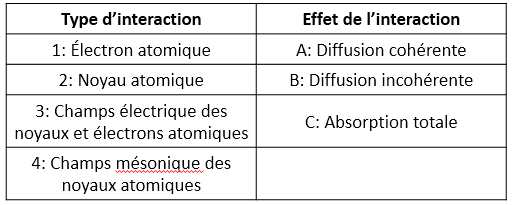
\includegraphics[scale=0.5]{ch4/image1}
	\captionof{table}{ }
	\end{wrapfigure}
La quantité de mouvement d'un photon vaut $\vec p = \hbar\vec{k}$ où $p = E_\gamma/c$ et $k$ est le
nombre d'onde. Ils interagissent avec la matière via des processus isolés, sans interactions entres-eux. 
Les photons sont des rayonnements \textbf{indirectement ionisants} : ils produisent des particules 
chargées qui, elles, vont ioniser la matière.\\

Pour des énergies entre le keV et le GeV, \textsc{Fano} a classifier 4 types d'interaction et 
3 conséquences de celle-ci, soit 12 processus théoriques possibles\footnote{Certains sont très 
rares, et d'autres n'ont jamais été observés.}. Sur ceux-ci, seuls trois effets dominent
\begin{enumerate}
\item \textit{L'effet Compton} (1B) : Le photon est diffusé par un électron libre ou faiblement lié.
La somme de l'énergie du photon et de l'énergie cinétique de l'électron est alors égale à l'énergie 
du photon incident
\item \textit{L'ffet photoélectrique} (1C) : Le photon est absorbé par un système électronique (atome). 
Il cède alors toute son énergie et un électron atomique\footnote{C'est-à-dire?} est éjecté hors de
l'atome avec une énergie cinétique égale à l'énergie du photon moins l'énergie de liaison de l'électron dans l'atome.

\item \textit{La création de paire} (3C) : Le photon disparait dans le champ électrique d'un noyau 
ou d'un électron et une paire électron-positron apparaît.
\end{enumerate}

Deux autres processus peuvent aussi jouer un rôle
\begin{enumerate}
\item \textit{Diffusion de Rayleigh} (1A) : Le photon est dévié sans perte d'énergie par un système
électronique (atome)
\item \textit{Photodésintégration du noyau}(2C): Le photon est absorbé par le noyau et une particule est émise ($\gamma, \alpha, p, n,\dots)$.
\end{enumerate}
On ne parlera pas du dernier point car l'énergie concernée est bien supérieure à celle utilisée en
métrologie nucléaire.


\subsection{Remarque importante}
Un photon \textbf{ne} peut \textbf{pas} être absorbé par un électron libre et lui céder toute son 
énergie. Par conservation de l'énergie et de l'impulsion avec $h\nu_0$ l'énergie du photo et $m,E$ et 
$p$, la masse, l'énergie totale et l'impulsion de l'électron on peut écrire
\begin{equation}
h\nu_0+mc^2=E,\qquad\qquad \dfrac{h\nu_0}{c}=p
\end{equation}
Ce qui implique que $E=pc+mc^2$. Or, par définition $E^2=p^2c^2+m^2c^4$. L'absorption serait possible
que pour $p=h\nu_0=0$ ce qui est à rejeter. 



\section{Effet Compton}%sl10
	\begin{wrapfigure}[6]{r}{4cm}
	\vspace{-10mm}
	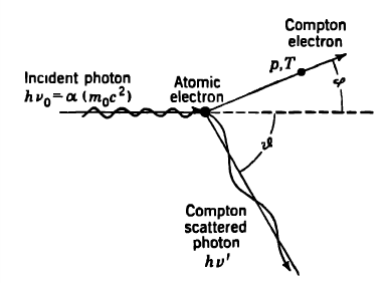
\includegraphics[scale=0.4]{ch4/image2}
	\captionof{figure}{ }
	\end{wrapfigure}
L'effet \textsc{Compton} est un scattering par un électron libre dans une certaine plage énergétique
où les électrons sont considérés comme libre\footnote{Lorsque ce n'est plus le cas, l'effet 
photoélectrique domine}. Le photon incident est donc diffusé (au sens du scattering) et cède une 
partie de son énergie à un électron.\\

C'est en \textit{1906} que \textsc{Thomson} calcula classiquement la section efficace de diffusion
d'une onde électromagnétique par un électron libre. Un électron oscille en réponse à la force
exercée par le champ électrique de l'onde, à la même fréquence que celui-ci. Il en résulte un 
dipôle magnétique faisant que l'électron rayonne causant une diffusion continue\footnote{L'idée 
est bonne, mais nous verrons que ceci est faux.} de l'onde incidente.\\

Pour une onde non polarisée, la section efficace de diffusion \textsc{Thomson} s'écrit
\begin{equation}
\frac{d\sigma_0}{d\Omega}=\frac{r_e^2}{2}(1+\cos^2\theta)
\end{equation}
où $r_e = e^2/4\pi\epsilon_0mc^2$, le rayon classique de l'électron. 

	
\subsection{Démonstration de Thomson}
Soit une onde électromagnétique de fréquence $\nu$ interagissant avec un électron libre de 
masse $m$ et charge $-e$
\begin{equation}
\overrightarrow{E}=E_0\exp{(i\overrightarrow{k}\overrightarrow{r}-i\nu t)}\overrightarrow{1_E}
\end{equation}
où $\vec{1_E}$ est la direction de polarisation. L'électron subit une force $\vec{F}$ à cause
de ce champ, son équation du mouvement s'écrit
\begin{equation}
m\frac{d^2\overrightarrow{r}}{dt^2}=-e\overrightarrow{E}
\end{equation}
Dans l'approximation dipolaire la puissance émise par unité d'angle solide s'écrit (formule 
de \textsc{Larmor} différentielle - voir cours d'électromagnétisme) 
\begin{equation}
\frac{dP}{d\Omega}=\frac{e^2}{16\pi^2\epsilon_0c^3}\langle a^2 \rangle \sin^2\Theta
\end{equation}
où $\Theta$ est l'angle entre la direction de polarisation et l'observateur. On peut directement
obtenir la moyenne de l'accélération au carré avec l'équation de mouvement
\begin{equation}
\langle a^2 \rangle=\frac{e^2}{2m^2}|E_0|^2
\end{equation}
En remplaçant dans la précédente équation, on trouve la puissance différentielle
\begin{equation}
\frac{dP}{d\Omega}=r_e^2 \frac{\epsilon_0c|E_0|^2}{2}\sin^2\Theta
\end{equation}
En considérant le module du vecteur de Poynting $I=\epsilon_0c\frac{|E_0|^2}{2}$ et en substituant
son expression, on trouve la section efficace différentielle
\begin{equation}
\frac{d\sigma_0}{d\Omega}=\frac{dP/d\Omega}{I}=r_e^2\sin^2\Theta
\end{equation}
Pour une onde incidente non-polarisée, il faut prendre la moyenne de $\Theta$
\begin{equation}
\overline{\sin^2\Theta}=\frac{1}{2}(1+\cos^2\theta)
\end{equation}
où $\theta$ est l'angle de scattering. En remplaçant on trouve l'équation de \textsc{Thomson}, 
purement classique
\begin{equation}
\frac{d\sigma_0}{d\Omega}=\frac{r_e^2}{2}(1+\cos^2\theta)
\end{equation}
L'intégration sur tout les angles possible donne la section efficace totale de diffusion
\textsc{Thomson}
\begin{equation}
\sigma_0=\frac{8\pi}{3}r_e^2=0.665\times 10^{-28} \mbox{~m}^2 \approx \frac{2}{3} \mbox{~~barn/\'electron}
\end{equation}
Le problème est la diffusion continue de l'onde incidente, comme \textsc{Compton} va faire remarquer.

\subsection{Expérience de Compton}%sl16
En \textit{1922}, \textsc{Compton} mesure les longueurs d'onde des rayonnements incidents et diffusés
et montre que le spectre n'est pas continu mais suit
\begin{equation}
\lambda_1-\lambda_0=\frac{h}{mc}(1-\cos\theta)
\end{equation}
où $\lambda_0, \lambda_1$ sont les longueurs d'ondes des photons incidents et diffusés et $\lambda_C$, 
la longueur d'onde de \textsc{Compton}. La diffusion par un électron ne dépend pas du nombre 
atomique du diffuseur, ni de la longueur de l'onde incidente :  l'énergie et l'impulsion perdue par
le photon se retrouvent dans un seul électron.

\subsubsection{Démonstration de l'expression de Compton}
Plaçons-nous dans le référentiel du laboratoire et écrivons les quadrivecteurs associés
\begin{eqnarray}
\mbox{photon avant} &\rightarrow& \left(\frac{h\nu_0}{c},\frac{h\nu_0}{c}\overrightarrow{n_0}\right)\\
\mbox{photon apr\`es} &\rightarrow& \left(\frac{h\nu_1}{c},\frac{h\nu_1}{c}\overrightarrow{n_1}\right)\\
\mbox{\'electron avant} &\rightarrow& \left(\frac{mc^2}{c},0\right)\\
\mbox{\'electron apr\`es} &\rightarrow& \left(\frac{E}{c},\overrightarrow{p}\right)
\end{eqnarray}
Par conservation de l'énergie et de l'impulsion
\begin{eqnarray}
h\nu_0+mc^2=h\nu_1+E\\
h\nu_0\overrightarrow{n_0}=h\nu_1\overrightarrow{n_1}+\overrightarrow{p}c
\end{eqnarray}
Avec $E^2=p^2c^2+m^2c^4$, en isolant $p$ :
\begin{equation}
(h(\nu_0-\nu_1)+mc^2)^2=h^2(\nu_0\overrightarrow{n_0}-\nu_1\overrightarrow{n_1})^2+m^2c^4
\end{equation}
Sachant que $\overrightarrow{n_0}\overrightarrow{n_1}=\cos{\theta}$, on trouve
\begin{equation}
h\nu_0\nu_1(1-\cos\theta)=mc^2(\nu_0-\nu_1)\Rightarrow \frac{hc^2}{\lambda_0\lambda_1}(1-\cos\theta)=mc^3\left(\frac{1}{\lambda_0}-\frac{1}{\lambda_1}\right)
\end{equation}
Et donc
\begin{equation}
\lambda_1-\lambda_0=\frac{h}{mc}(1-\cos\theta)
\end{equation}

\subsection{Relations entre énergies et angles}%sl19
Soit $E_0$ et $E_1$ les énergies du photon indicent et diffusé, $T=E_0-E_1$ l'énergie cinétique 
cédée à l'électron, $\theta$ l'angle de diffusion du photo, $\phi$ l'angle entre la trajectoire de
l'électron et la direction initiale du photon et $\alpha=E_0/mc^2$. On peut écrire
\begin{equation}
T=E_0\frac{2\alpha \cos^2\phi}{(1+\alpha)^2-\alpha^2\cos^2\phi}=E_0\frac{\alpha(1-\cos\theta)}{1+\alpha(1-\cos\theta)}
\end{equation}\ 

	\begin{wrapfigure}[14]{l}{8.5cm}
	\vspace{5mm}
	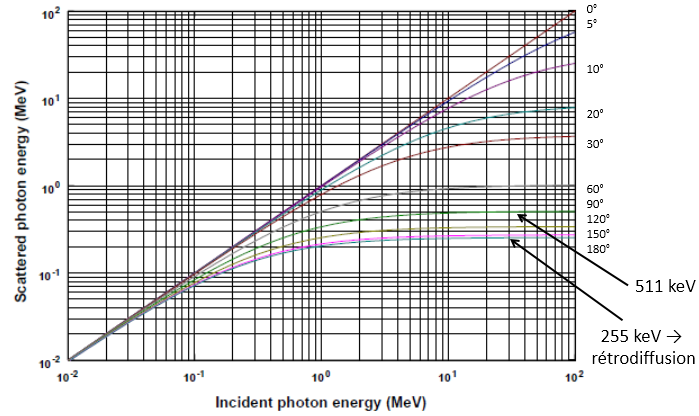
\includegraphics[scale=0.45]{ch4/image3}
	\captionof{figure}{ }
	\end{wrapfigure}
	\ 
	
\begin{equation}
E_1=E_0\frac{1}{1+\alpha (1-\cos\theta)},\quad 
\cot\phi=(1+\alpha)\tan\frac{\theta}{2}
\end{equation}

Ces formules représentées graphiquement donnent déjà un bon nombre d'informations. Comme $0<\theta<
\pi$, on sait que $(E_1)_{min} = E_0/(1+2\alpha)$ et $(E_1)_{max} : E_0$. Lorsque l'angle augmente, 
$E_1$ a tendance à diminuer. L'effet de l'angle se marque assez peu à faible énergie mais devient
significatif à haute énergie. La ligne bleue correspond à une rétro-diffusion, ce point sera
abordé plus tard.

\newpage
\textsc{Remarques}
\begin{itemize}
\item[$\bullet$] Le déplacement en longueur d'onde ne dépend pas de l'énergie du photon incident 
(uniquement de l'angle de diffusion)
\item[$\bullet$] Le déplacement en énergie dépend fortement de l'énergie du photon incident et 
augmente fortement avec l'énergie
\item[$\bullet$] Pour $E_0$ petit, le photon perd peu d'énergie $\forall\theta$
\item[$\bullet$] Lorsque $E_0$ augmente, la variation de l'énergie du photon diffusé avec l'angle
 devient de plus en plus rapide
\item[$\bullet$] A $90^\circ$, $E_1 < 511$ keV (toujours, =$mc^2$)
\item[$\bullet$] A $180^\circ$, $E_1 < 255$ keV (toujours, =$mc^2/2$). Il s'agit de la
rétro-diffusion du photon et explique le pic de rétro-diffusion dans les spectres $\gamma$.
\end{itemize}\ 

	\begin{wrapfigure}[8]{r}{6cm}
	\vspace{-7mm}
	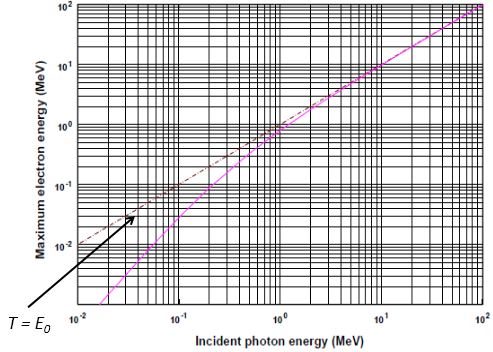
\includegraphics[scale=0.5]{ch4/image4}
	\captionof{figure}{ }
	\end{wrapfigure}
	
Regardons $\phi$. On observe que $0<\phi<\pi/2$ impliquant $T_{min}=0$ et \\

\retenir{\begin{equation}
T_{max} = \dfrac{E_0}{1+(1/2\alpha)}
\end{equation}
A retenir car pratique pour tracer des spectres!}\ \\

Ci-contre, la représentation de la variation de l'énergie maximale de l'électron en fonction 
de l'énergie du photon indicent. On remarque que la déviation du photon se fait dans le sens
de la trajectoire pour les grandes énergies (et donc faible angle).\\



\subsection{Section efficace différentielle angulaire, énergétique et totale}
\subsubsection{Section efficace différentielle angulaire} %sl25
Il s'agit de la première chose qui a été calculé par \textsc{Klein-Nishina} (valable pour 
des électrons libres et au repos) via la théorie quantique relativise et l'équation de
\textsc{Dirac}.

\begin{center}
	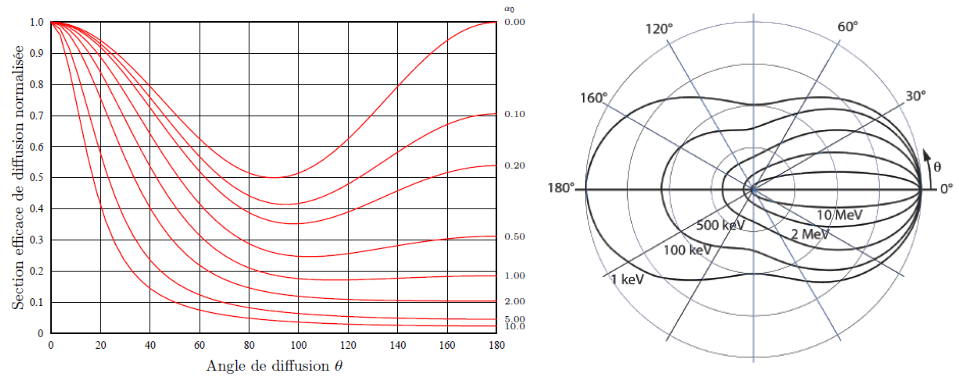
\includegraphics[scale=0.6]{ch4/image5}
	\captionof{figure}{Plus on monte en énergie, plusla direction privilégiée est dnas le sens de la trajectoire (droite).}
\end{center}

\newpage
La section efficace différentielle de diffusion d'un photon (non polarisé) par un électron dans
l'angle solide d$\Omega$ autour de la direction formant un angle $\theta$ avec la direction initiale
du photon est donnée par 
\begin{equation}
\frac{d\sigma}{d\Omega}=\frac{r_e^2}{2}\left(\frac{\nu'}{\nu_0}\right)\left(\frac{\nu_0}{\nu'}+\frac{\nu'}{\nu_0}-\sin^2\theta\right)
\end{equation}
où $r_e$ est le rayon classique de l'électron. Notons la non-dépendance en $Z$. Pour de très faibles
énergie ($\alpha\ll 1$), $E_1\approx E_0$ impliquant que d$\sigma \approx$ d$\sigma_0$ : on 
retrouve la section efficace de \textsc{Thomson} ! Celle-ci n'était donc pas si mauvaise car on la
retrouve à faible énergie.

\subsubsection{Section efficace différentielle énergétique}%sl28
A partir de la section efficace différentielle en angle, on peut trouver les sections différentielles
en énergie. Rien de compliqué, mais rien de drôle non plus
\begin{equation}
\frac{d\sigma}{dE_1}=\frac{\pi r_e^2}{\alpha^2m_ec^2}\left\{2+\left(\frac{E_0-E_1}{E_1}\right)^2\left[\frac{1}{\alpha^2}+\frac{E_1}{E_0}-\frac{2}{\alpha}\left(\frac{E_1}{E_0-E_1}\right) \right]\right\}
\end{equation}
Par changement de variable (à faire un samedi soir)
\begin{equation}
\frac{d\sigma}{dT}=\frac{\pi r_e^2}{\alpha^2m_ec^2}\left\{2+\left(\frac{T}{E_0-T}\right)^2\left[\frac{1}{\alpha^2}+\frac{E_0-T}{E_0}-\frac{2}{\alpha}\left(\frac{E_0-T}{T}\right) \right]\right\}
\end{equation}
La représentation graphique (slide 29) montre que cette section efficace est assez équiprobable pour
de faibles énergies. Plus l'énergie augmente, plus il y a un pic prononcé lorsque l'on arrive à
la valeur du seuil \textsc{Compton}.

\subsubsection{Section efficace différentielle totale}%sl30
Après intégration de la section efficace de \textsc{Klein-Nishina} sur les angles
\begin{equation}
\sigma=2\pi r_e^2\left\{\frac{1+\alpha}{\alpha^2}\left[\frac{2(1+\alpha)}{1+2\alpha}-\frac{\ln{(1+2\alpha)}}{\alpha}\right]+\frac{\ln{(1+2\alpha)}}{2\alpha}-\frac{1+3\alpha}{(1+2\alpha)^2}\right\}
\end{equation}
Pour $\alpha\ll 1 \to \sigma \approx \sigma_0$, la section efficace de \textsc{Thomson}. Pour
$\alpha\gg 1, \sigma  \to (\ln\alpha)/\alpha$, la section efficace de \textsc{Compton} décroit
lorsque l'énergie du photon augmente. Si on regarde les précédents graphique, la distribution
est piquée en $\theta=0$ ce qui répond au cas où il n'y a ni diffusion, ni transfert d'énergie et
donc pas d'effet. Notons que la section efficace \textbf{atomique} est proportionnelle à $Z$.\\

La section efficace $\sigma$ représente la probabilité de collision, soit le cas où une partie de
l'énergie est diffusée et l'autre est cédée à l'électron (absorbée). La collision reprend donc 
la diffusion, mais également l'absorption. Pour caractériser cet aspect, on défini une section
efficace de diffusion $\sigma_s$ et d'absorption $\sigma_a$ tel que $\sigma = \sigma_s+\sigma_a$.



\subsection{Diffusion cohérente et incohérente}%sl32

Pour de très faibles énergies $E_0$, d'électron est de moins en moins libre/au repos et les anciennes 
hypothèses tombent à l'eau, il va falloir prendre en considération le système électronique tout
entier et non plus . Deux cas sont possibles
\begin{enumerate}
\item L'atome reste dans son état intial et le photo est juste dévie : diffusion de 
\textsc{Rayleigh} (\textbf{cohérente})
\item L'atome change d'état : le photon perd de l'énergie, la diffusion est \textbf{incohérente}
\end{enumerate}
Pour de grandes énergies, on nomme la diffusion incohérente la diffusion \textsc{Compton}.\\

	\begin{wrapfigure}[15]{r}{8cm}
	\vspace{-5mm}
	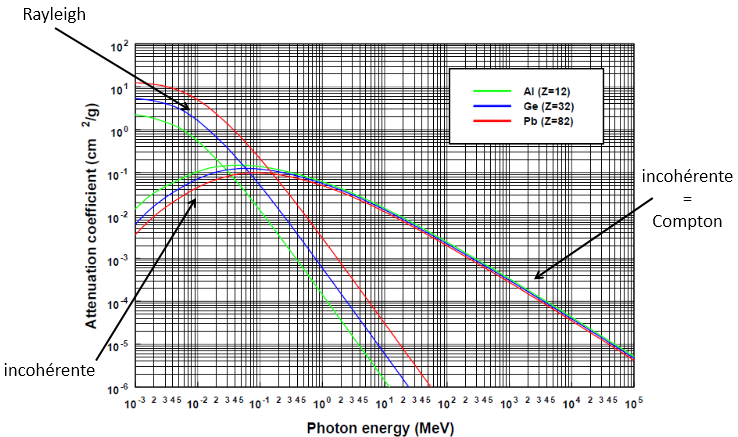
\includegraphics[scale=0.5]{ch4/image6}
	\captionof{figure}{ }
	\end{wrapfigure}
	
En guise de première approximation pour la diffusion cohérente, on peut voir le système électronique
comme un système de charge $Ze$ et de masse $Zm$. La section efficace de Rayleigh vaut alors
\begin{equation}
_a\sigma_{coh}=Z^2\sigma_0
\end{equation}
En réalité la structure du nuage électronique implique une diminution de la diffusion et l'on utilise
\begin{equation}
_a\sigma_{coh}=F^2\sigma_0
\end{equation}
Pour la diffusion incohérente, on modifie la section efficace de \textsc{Klein-Nishina} en 
introduisant la fonction de diffusion incohérente $S$ tenant compte du fait qu'un 
photon peut éjecter un électron
\begin{equation}
_a\sigma_{incoh}=Z\sigma S
\end{equation}


\section{Effet photoélectrique}%sl38
	\begin{wrapfigure}[7]{l}{5cm}
	\vspace{-5mm}
	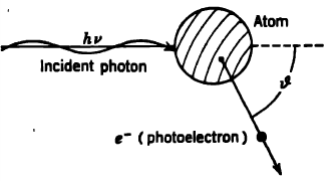
\includegraphics[scale=0.5]{ch4/image7}
	\captionof{figure}{ }
	\end{wrapfigure}
L'\textbf{effet photoélectrique} est un processus au cours duquel un photon incident interagit avec 
un atome et éjecte un électron (processus expliqué correctement par \textsc{Einstein} en 
\textit{1905}), souvent appelé \textit{photoélectron}. Ce processus de capture d'un photon par un
atome dont un électron est excité dans un état continu est le processus inverse de l'émission spontanée d'un photon par un atome excité


\subsection{Conservation de l'énergie et énergie de liaison} %sl39
	\begin{wrapfigure}[15]{r}{7cm}
	\vspace{-5mm}
	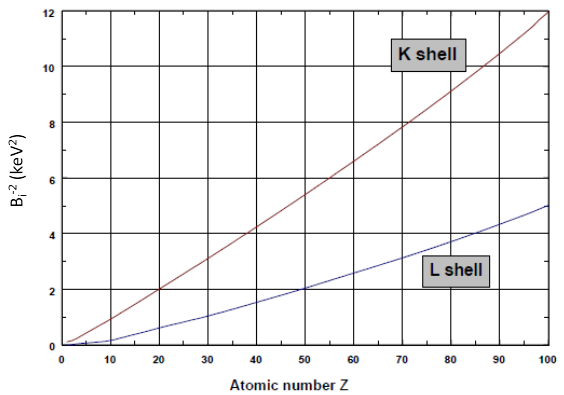
\includegraphics[scale=0.5]{ch4/image8}
	\captionof{figure}{Pour $Z > 30$, les énergies de liaison obéissent approximativement à 
	$B_i = a_i(Z-c_i)^2$ (avec $a_i$ et $c_i$, des constantes pour chaque couche)}
	\end{wrapfigure}
Soit l'absorption totale d'un photon d'énergie $h\nu_0$ causant l'émission d'un électron avec une
énergie cinétique $T$ hors d'une couché atomique caractérisée par une énergie de liaison $B_i$. En
négligeant l'énergie du recul du noyau
\begin{equation}
h\nu_0=T+B_i
\end{equation}
Par conservation, il faut que $h\nu_0>B_i$. Ainsi lorsque $h\nu_0$ augmente, la probabilité de l'effet
photoélectrique diminue car le comportement de l'électron se rapproche plus de celui d'un électron
libre (et celui-ci \textbf{ne} peut \textbf{pas} se faire totalement absorbé). A priori on regarde 
plus les couches externes (couche $K\to B_K$), ceux-ci possédant une énergie de liaison plus faible.

\newpage
\subsection{Section efficace}%sl41
On peut décomposer la section efficace par atome $_a\tau$ en une somme de sections efficaces 
partielles $_a\tau_i$ correspondant à l'éjection d'une électron hors d'une couche $i$
\begin{equation}
_a\tau=\sum_i {}_a\tau_i
\end{equation}	
Le calcul de $_a\tau_K$ a été fait pour un atome hydrogénoïde dans 	l'approximation de \textsc{Born}
en utilisant une onde plane comme fonction d'onde de l'électron éjecté : pas le choix, la fonction
d'onde de l'électron est trop compliquée. Restreignons la zone de travail en énergie en faisant
l'approximation non relativiste et que l'interaction noyau/électron est négligeable : $\B_k\ll 
\hbar\nu_0\ll mc^2$. On trouve (cadeau)
\begin{equation}
_a\tau_K=\frac{8\pi}{3}\left(\frac{a_0}{Z}\right)^232\alpha\left(\frac{B_K}{h\nu_0}\right)^{7/2}
\end{equation}
Lorsque l'approximation de \textsc{Born} n'est plus valable, il faut introduire un facteur correctif
\begin{equation}
f(\xi)=2\pi\left(\frac{B_K}{h\nu_0}\right)^{1/2}\frac{e^{-4\xi \text{arccot}{\xi}}}{1-e^{-2\pi \xi}}\mbox{~~avec~~}\xi=\left(\frac{B_K}{h\nu_0-B_K}\right)^{1/2}
\end{equation}
En pratique pas grand monde s'intéresse à ceci, même ceux qui travaillent dans le domaine 
utilisent les valeurs de tables et ne font pas trop attention à la forme. Ce qui est intéressant
c'est que $a_0/Z$ est grossièrement la dimension de l'atome et que l'énergie varie en 
$h\nu_0^{7/2}$.\\


	\begin{wrapfigure}[10]{r}{7cm}
	\vspace{-5mm}
	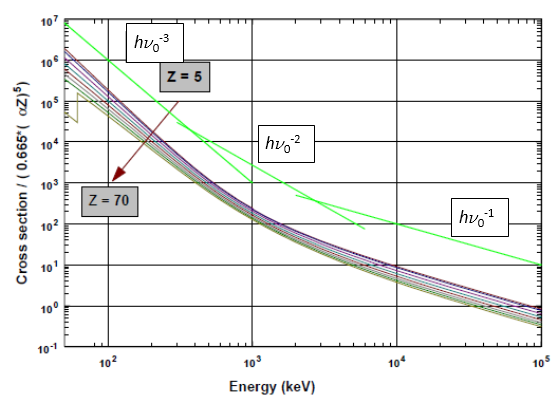
\includegraphics[scale=0.5]{ch4/image9}
	\captionof{figure}{Variation de $_a\tau$ avec $h\nu_0$}
	\end{wrapfigure}
	
Les autres section efficaces partielles suivent le même comportement, on les note sous la forme\\

\retenir{
\begin{equation}
_a\tau=C\frac{Z^n}{(h\nu_0)^k}
\end{equation}
où $4<n<4.6$ et $1<k<3$.}\ \\

Cette formule est intéressante à retenir car elle montre une forte dépendance en énergie mais 
également une dépendance en $Z$. Ces constantes sont difficile à trouver, on sait que l'énergie 
doit être en proche (en puissance) de $-7/2$ mais on en sait pas plus. 


\subsection{Distribution angulaire des photoélectrons}
On se rappelle que - dans l'approximation de \textsc{Born} - la section efficace différentielle
est proportionnelle à
\begin{equation}
f(\theta)=\frac{\sin^2\theta}{(1-\beta\cos\theta)^4}
\end{equation}
La section efficace s'annule dans la direction du photon indicent $\theta=0$ ce qui est une 
conséquence de la nature transverse des ondes électromagnétiques. L'électron tend donc à être
éjecté dans la direction du champ $\vec{E}$ de cette onde\footnote{Notons que, physiquement, 
$\theta=0$ est impossible.}. Dans le cas relativiste
\begin{equation}
f(\theta)=\frac{\sin^2\theta}{(1-\beta\cos\theta)^4}+\frac{3(1-\sqrt{1-\beta^2})-2\beta^2}{2(1-\beta^2)^{3/2}}\times\frac{\sin^2\theta}{(1-\beta\cos\theta)^3}
\end{equation}
\newpage
	\begin{wrapfigure}[7]{r}{4.5cm}
	\vspace{-3mm}
	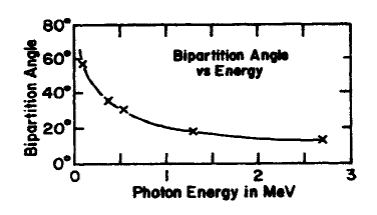
\includegraphics[scale=0.5]{ch4/image10}
	\captionof{figure}{ }
	\end{wrapfigure}

Que ce soit relativiste ou non, lorsque l'énergie des photons augmente de plus en plus d'électrons
sont éjectés vers l'avant. \\

On nomme \textbf{angle de bipartition} $\theta_b$ l'angle pour lequel la moitié des photoélectrons
sont émis vers l'avant dans un cône de demi-angle inférieur à $\theta_b$.



\subsection{Phénomène consécutif à l'effet photoélectrique}%sl53
	\begin{wrapfigure}[9]{l}{9.8cm}
	\vspace{-5mm}
	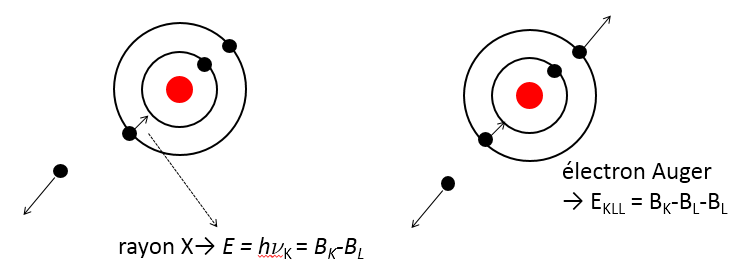
\includegraphics[scale=0.5]{ch4/image11}
	\captionof{figure}{ }
	\end{wrapfigure}
L'émission d'un électron à cause d'un photoélectrique crée un trou dans une couche interne. Après
réarrangement électronique, il y a émission d'un rayon $X$ (fluorescence) \textit{ou} d'un électron
\textsc{Auger}. On défini alors un \textbf{rendement de fluorescence} $\omega_i$ qui est la 
probabilité d'émission d'un photon après une transition vers la couche $i$. Ce rendement est faible
pour les matériaux à petit $Z$.


\section{Création de paire}%sl 55
	\begin{wrapfigure}[5]{r}{5.6cm}
	\vspace{-5mm}
	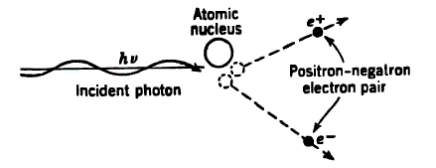
\includegraphics[scale=0.5]{ch4/image12}
	\captionof{figure}{ }
	\end{wrapfigure}
La création de paire se produit dans le champ électrique du noyau ou d'un électron atomique (plus 
rarement, on parlera de création de triplet où une partie de l'énergie est transférée à l'électron
initial)), le photon disparaît alors et il se forme une paire
électron-positron. 

\subsection{Lois de conservation}%sl56
Afin de déterminer l'énergie minimale du photon incident pour avoir création de paire, écrivons 
les équations de conservation. Avant l'interaction, on travaille dans le repère de la particule
cible de masse $M$, au repos
\begin{eqnarray}
\mbox{photon avant} &\rightarrow& \left(\frac{h\nu_0}{c},\frac{h\nu_0}{c}\right)\\
\mbox{particule cible avant} &\rightarrow& \left(\frac{Mc^2}{c},0\right)
\end{eqnarray}
Après l'interaction, on se place dans le référentiel du centre de masse
\begin{eqnarray}
\mbox{\'electron apr\`es} &\rightarrow& \left(\frac{mc^2+T_e}{c},\overrightarrow{p_e}\right)\\
\mbox{positron apr\`es} &\rightarrow& \left(\frac{mc^2+T_p}{c},\overrightarrow{p_p}\right)\\
\mbox{particule cible apr\`es} &\rightarrow& \left(\frac{Mc^2+T_C}{c},\overrightarrow{p_C}\right)
\end{eqnarray}
Après le choc, en travaillant dans le référentiel du centre de masse\footnote{Égalité nulle car
init. au repos?}
\begin{equation}
\overrightarrow{p_e}+\overrightarrow{p_p}+\overrightarrow{p_C}=0
\end{equation}
En notant $T_{tot} = T_e+T_p+T_C$ et par conservation de l'invariant $P^2=(E/c)^2+p^2$
\begin{eqnarray}
\mbox{avant} &\rightarrow& P^2=\left(\frac{h\nu_0}{c}+\frac{Mc^2}{c}\right)^2-\left(\frac{h\nu_0}{c}\right)^2\\
\mbox{apr\`es} &\rightarrow& P^2=\left(\frac{2mc^2+Mc^2+T_{tot}}{c}\right)^2
\end{eqnarray}
On trouve l'énergie minimale $h\nu_{m,min}$ en égalant les deux expression pour $T_{tot}=0$
\begin{equation}
h\nu_{0,min}=2mc^2\left(1+\frac{m}{M}\right)
\end{equation}
où $m$ est la masse de l'électron et $M$ celle de la particule cible
En conclusion
\begin{itemize}
\item[$\bullet$] \textit{Dans le champ d'un noyau} : $M\gg m \to h\nu_{0,min} = 2mc^2$
\item[$\bullet$] \textit{Dans le champ d'un électron} : $M= m \to h\nu_{0,min} = 4mc^2$
\end{itemize}
Ce phénomène est aussi possible entre $2mc^2$ et $4mc^2$ car l'atome peut prendre avec lui
une fraction de la quantité de mouvement initiale, mais c'est très rare.

\subsection{Section efficace dans le champ d'un noyau}%sl59
Le calcul de la section efficace \textsc{Compton} était déjà sympathique, ici c'est pire. On se
contentera de donner les résultats important sans faire de calculs détaillés. La raison est que 
c'est compliqué notamment à cause du nuage électronique qui a des effets d'écrantage des électrons
atomiques. \\

Lorsqu'on regarde les spectres de l'électron et du positron, ils sont décalés. On peut négliger cette
différence et considérer la section efficace différentielle pour la création d'un électron à énergie
cinétique $T_-$ est identique à celle de création d'un positron à énergie cinétique $T_+=h\nu_0-2mc-
T_-$. Cette section efficace différentielle est symétrique par rapport à 
\begin{equation}
\langle T \rangle = \frac{h\nu_{0}-2mc^2}{2}
\end{equation}
En s'amusant un peu
\begin{equation}
\frac{d{}_a\kappa}{dT_+}=\frac{\sigma_pZ^2P(T_+,h\nu_0,Z)}{h\nu_0-2mc^2}{\mbox{~~~~pour~~~~}}h\nu_0>2m_ec^2
\end{equation}
où encore
\begin{equation}
\frac{d{}_a\kappa}{dx}=\sigma_pZ^2P(x,h\nu_0,Z)
\end{equation}
avec $x = T_+/(h\nu_0-2m_ec^2)$.\\

	\begin{wrapfigure}[6]{r}{3cm}
	\vspace{-5mm}
	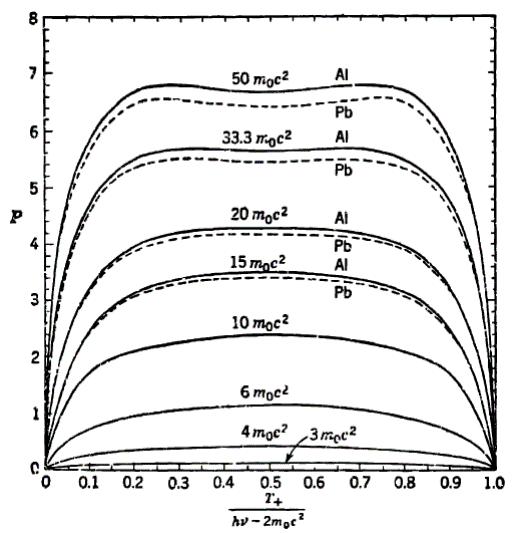
\includegraphics[scale=0.24]{ch4/image13}
	\captionof{figure}{ }
	\end{wrapfigure}
Intéressons-nous quelque peu à la fonction $P(x,h\nu_0,Z)$ représentée ci-contre. Il s'agit d'une
fonction symétrique qui ne dépend que peu de $Z$ : la section efficace est $\propto Z^2$. Cette 
fonction est lentement variable en l'énergie $h\nu_0$ du photon et est approximativement constante
pour $0.2<x<0.8$.

\newpage
\subsection{Section efficace totale}%sl63	
Si on veut la section efficace totale, il faut intégrer sur l'énergie $T_+$
\begin{eqnarray}
{}_a\kappa&=&\int_{T_+}d{}_a\kappa=\sigma_pZ^2\int_0^{h\nu_0-2mc^2}\frac{PdT_+}{h\nu_0-2mc^2}\\
&=&\sigma_pZ^2\int_0^{1}Pd\left(\frac{T_+}{h\nu_0-2mc^2}\right)\\
&=&\sigma_pZ^2\langle P\rangle
\end{eqnarray}
où $\langle P\rangle$ est la valeur moyenne de $P$. Celle-ci dépend très peu de $Z$ est est 
une fonction lentement croissante de $h\nu_0$ avant de devenir constante à grande énergie 
(>100 MeV) à cause de l'écrantage.




\subsection{Section efficace dans la champ d'un électron}
Le calcul est très compliqué mais on peut montrer que
\begin{equation}
{}_a\kappa_{triplet}=\sigma_pZ\langle P\rangle_{triplet}{\mbox{~~~~pour~~~~}}h\nu_0>4m_ec^2
\end{equation}
et donc que
\begin{equation}
\frac{{}_a\kappa_{triplet}}{{}_a\kappa}\simeq \frac{1}{CZ}
\end{equation}
où $C$ est un paramètre seulement fonction de $h\nu_0$. Ce qui est important c'est que 
la création de paire dans le champ des électrons ne contribue que peu à la section efficace 
totale de création de paire sauf pour les matériaux à $Z$ petit 

\subsection{Direction d'émission de la paire électron-positron}%sl67
	\begin{wrapfigure}[6]{l}{6cm}
	\vspace{-5mm}
	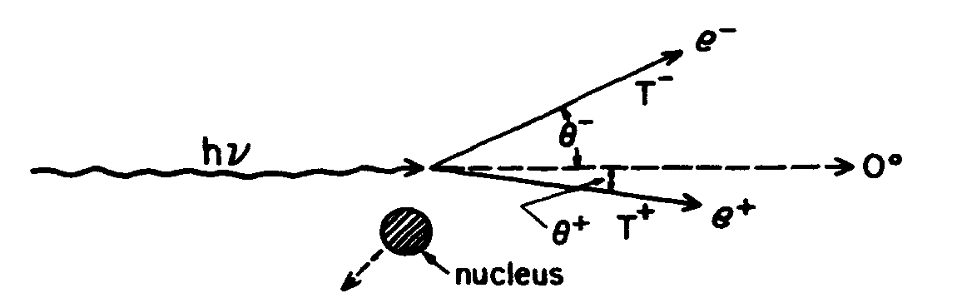
\includegraphics[scale=0.24]{ch4/image14}
	\captionof{figure}{ }
	\end{wrapfigure}
	
Pour des photons d'énergie $h\nu_0$ largement supérieur à l'énergie de seuil, les électrons et 
positrons sont fortement émis vers l'avant. Leur angle d'émission moyen relatif à la direction
d'origine du photon vont grossièrement (rad.)
\begin{equation}
\langle \theta \rangle \simeq \frac{mc^2}{\langle T \rangle}
\end{equation}






\subsection{Phénomène consécutif à la création de paire et photodésintégration du noyau} 
\subsubsection{Phénomène consécutif à la création de paire}
Très brièvement, le positron s'annihile avec un électron (au repos) lorsqu'il traverse la matière mais 
avant ça il ralenti car les collisions sont nettement plus probables que l'annihilation. Cette
dernière se produit le plus souvent lorsque le positron est \textit{quasi au repos} et deux 
photons de 511 keV sont produits à 108$^\circ$ l'un de l'autre.

\subsubsection{Photodésintégration du noyau}
Le photon est absorbé par un noyau et une particule est émise (un photon ou une particule légère (p,
n,$\alpha$, \dots) mais il faut une énergie entre 8 et 20 MeV(!).

\subsection{Comparaison des différents effets}
Commenter le graphique est une bonne question d'examen. Voir notes, slide 70 (beaucoup à dire, je 
n'ai pas le temps de le faire pour le moment).


\section{Coefficient d'atténuation}
Nous venons de voir trois processus d'interaction d'un photon dans la matière et leurs sections
efficaces
\begin{enumerate}
\item Effet photoélectrique : $_a\tau$
\item Effet \textsc{Compton} : $_a\sigma = Z\sigma$
\item Création de paire : $_a\kappa$
\end{enumerate}
où $_a$ signifie atomique. Les autres processus étant négligeable, la section efficace totale
n'est que la somme de ces trois effets
\begin{equation}
{}_a\mu={}_a\tau+{}_a\sigma+{}_a\kappa
\end{equation}
La probabilité qu'un photon ait une interaction dans une cible mince de densité $N$ et d'épaisseur
$dx$ vaut $_a\mu Ndx$. Pour un faisceau monocinétique de $I$ photons par unité de temps, le taux 
de collision vaut $I_a\mu Ndx$. La variation d$I$ d'intensité après avoir quitté la cible vaut 
alors $dI = -I_a\mu Ndx$. Pour une cible finie et un faisceau initial perpendiculaire à la cible
de $I_0$ particules, l'intensité après le passage dans la cible est
\begin{equation}
I=I_0\exp{(-_a\mu Nl)}
\end{equation}
où $\mu = _a\mu N$ est le \textbf{coefficient linéique d'atténuation} (m$^{-1}$) qui nous 
informe sur la \textit{fréquence des collisions}.

\subsection{Géométrie à faisceau étroit}
	\begin{wrapfigure}[9]{l}{7cm}
	\vspace{-5mm}
	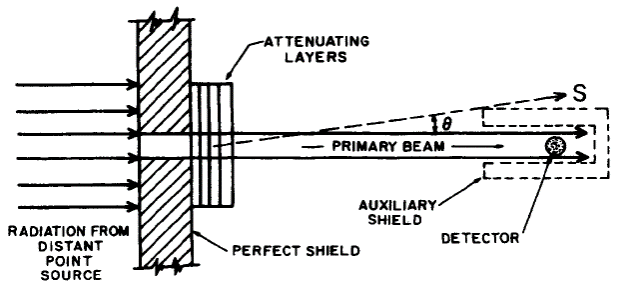
\includegraphics[scale=0.4]{ch4/image16}
	\captionof{figure}{ }
	\end{wrapfigure}
Pour vérifier cette loi, il faut utiliser une \textit{géométrie à faisceau étroit} empêchant les
qui empêche les particules primaires déviées et les secondaires d'attendre le détecteur (on 
ne veut pas qu'un électron arraché à la cible soit détectée). Pour se faire il faut une grande 
distance entre la source et l'atténuateur, de même entre l'atténuateur et le détecteur et le 
faisceau doit recouvrir tout le détecteur uniformément. De même, on utilise un blindage devant
l'atténuateur pour stopper les rayons incident exceptés ceux passant par l'ouverture et un 
blindage autour du détecteur pour stopper les rayons $X$ ou $\gamma$.

\subsection{Coefficient massique d'atténuation}%78
On définit le \textbf{coefficient massique d'atténuation} comme le rapport $\rho/\mu$ 
(m$^2$.kg$^{-1}$). Il s'agit du quotient de $dI/I$ par $\rho dI$ où $dI/I$ est la fraction de
particules indirectement ionisantes qui subissent des interactions le long de la distance d$l$ 
parcourue dans un matériau de masse volumique $\rho$. Il s'agit du coefficient \textbf{le plus
important}.\\

Il s'agit d'un coefficient global qui prend en compte les interactions des particules dans la 
matière sans préciser la nature de l'interaction. Ils sont directement proportionnel à la 
section efficace et ne dépendent \textbf{pas} de la nature de la cible !

\newpage
Si le matériau contient plusieurs espèces atomiques, on somme les probabilités d'interaction 
de chaque type d'atomes. Le coefficient massique d'atténuation total est alors donén par
\begin{equation}
\left(\frac{\mu}{\rho}\right)=\left(\frac{\mu}{\rho}\right)_1w_1+\left(\frac{\mu}{\rho}\right)_2w_2+
\dots
\end{equation}
où $w_i$ sont les fractions massiques des différentes espèces d'atomes.

\subsection{Coefficient de transfert massique d'énergie}%sl83
Le coefficient d'atténuation massique mesure le nombre moyen d'interaction entre un photon 
et la matière, il permet donc d'évaluer la fréquence des collisions. Souvent on s'intéresse
à l'énergie déposée "localement"\footnote{Ici quasi uniquement dues aux effets des électrons 
produits.}. On définit alors le \textbf{coefficient de transfert massique d'énergie} $\mu_{tr}/\rho$.
On le défini aussi comme\footnote{Voir slide 84 pour plus de détails, peu de notes}
\begin{equation}
\frac{\mu_{tr}}{\rho}=f_{ph}\frac{\tau}{\rho}+f_{C}\frac{\sigma}{\rho}+f_{pn}\frac{\kappa_n}{\rho}+f_{pe}\frac{\kappa_e}{\rho}
\end{equation}
avec $f_i$, les fractions d'énergie du photon transférées sous forme d'énergie cinétique à des
particules chargées pour chaque processus. Pour les trois processus étudiés
\begin{enumerate}
\item Effet photoélectrique
\begin{equation}
f_{ph}=1-\frac{E_X}{E}
\end{equation}
où $E_X$ est l'énergie moyenne des photons de fluorescence. Tout l'énergie est cédée à l'électron, 
sauf celle cédée au rayon $X$.
\item Effet \textsc{Compton}
\begin{equation}
f_{C}=1-\frac{\langle E_1 \rangle +E_X}{E}
\end{equation}
avec $\langle E_1\rangle$ l'énergie du photon diffusé. Il s'agit de (ce qui est émis)-(ce qui est
diffusé). Notons que le $E_X$ peut être négligé en pratique. 
\item Création de paire
\begin{equation}
f_{pn}=1-\frac{2mc^2}{E},\qquad\qquad\qquad f_{pe}=1-\frac{2mc^2+E_X}{E}
\end{equation}
(Tout)-(énergie servant à créer la paire). Ici on ne peut pas négliger le rayon $X$ car ça dépend
ou s'est formée la paire (alors que \textsc{Compton} concernait les électrons moins liés).
\end{enumerate}\ \\

Une fraction de l'énergie cinétique emportée par les particules chargées mises en mouvement lors des
interactions des particules primaires avec le matériau peut ne pas être absorbée localement. Une
partie de leur énergie peut alors être émise sous forme de rayonnement de freinage (surtout pour des 
électrons secondaires d'énergie élevée). Il faut alors corriger le précédent coefficient pour tenir
compte de ces rayonnements
\begin{equation}
 \frac{\mu_{en}}{\rho}=(1-g)\frac{\mu_{tr}}{\rho}
\end{equation}
où $g$ est la fraction de l'énergie des particules secondaires chargées perdue sous la forme de 
rayonnement de freinage dans le matériau. Ceci n'a de différence significative que pour des 
$\gamma$ d'énergie élevés que pour provoquer le rayonnement de freinage (surtout matériau à $Z$ 
élevé).\\

Le schéma 90 est une bonne question d'examen pour s'assurer que tout est clair, il n'est pas
commenté ici.